\section{Application: Systems of linear differential equations}

% ----------------------------------------------------------------------
\subsection{Linear differential equations}

Recall from calculus that if $y=f(x)$ is a function, then $y' = f'(x)$
is its derivative%
\index{derivative} and $y'' = f''(x)$ is its second derivative.  For
example,
\begin{equation*}
  \begin{array}{c@{~}c@{~}c}
    y &=& \sin(x),\\
    y' &=& \cos(x),\\
    y''&=& -\sin(x).\\
  \end{array}
\end{equation*}
Note that if $y=\sin(x)$, the second derivative $y''$ is exactly the
negative of $y$, i.e.,
\begin{equation*}
  y'' = -y.
\end{equation*}
This last equation is called a \textbf{differential equation}%
\index{equation!differential|see{differential equation}}%
\index{differential equation}. Unlike an ordinary equation, which is
about an unknown {\em number}, a differential equation is about an
unknown {\em function}. Typically, a differential equation mentions
the function and one or more of its derivatives. A differential
equation that only mentions the first derivative $y'$ is called a
\textbf{first-order}%
\index{differential equation!first order} differential equation. A
differential equation that also mentions the second derivative $y''$
is called a \textbf{second-order}%
\index{differential equation!second order} differential equation.
If the equation is a linear function of $y$ and its derivatives, it is
called a \textbf{linear differential equation}%
\index{linear differential equation}%
\index{differential equation!linear}.

We say that the function $y=\sin(x)$ is a \textbf{solution}%
\index{differential equation!solution} of the differential equation
$y'' = -y$. It is not the only solution. Another solution is
$y=\cos(x)$, because in that case, $y''=-\cos(x)$, and therefore
$y''=-y$. From calculus, we know that the \textbf{general solution} to
the differential equation $y'' = -y$ is given by
\begin{equation*}
  y = a\sin(x) + b\cos(x),
\end{equation*}
where $a$ and $b$ are any real numbers, i.e., parameters. Using the
terminology of linear algebra, we can say that the general solution of
the equation $y'' = -y$ is a \textbf{linear combination}%
\index{linear combination!of basic solutions!of differential equation}
of the \textbf{basic solutions}%
\index{basic solution!of differential equation}%
\index{differential equation!basic solution} $y=\sin(x)$ and
$y=\cos(x)$. More generally, we have the following theorem from
calculus:

\begin{theorem}{Solutions of $y''=-qy$}{differential-equation}
  Let $q$ be a positive real number.  The differential equation
  \begin{equation*}
    \begin{array}{l@{~~}l@{~}clllll}
    y'' &=& -qy &\quad\mbox{has basic solutions}\quad\quad &
    y = \sin(\sqrt{q}\,x) & \mbox{and} & y = \cos(\sqrt{q}\,x),\\
    y'' &=& 0 &\quad\mbox{has basic solutions}\quad\quad &
    y = 1 & \mbox{and} & y = x, \\
    y'' &=& qy &\quad\mbox{has basic solutions}\quad\quad &
    y = e^{\sqrt{q}\,x} & \mbox{and} & y = e^{-\sqrt{q}\,x}. \\
    \end{array}
  \end{equation*}
\end{theorem}

\begin{proof}
  By taking derivatives, it is easy to check that each of the six
  functions is a solution of the corresponding differential
  equation. For example, for $y=\sin(\sqrt{q}\,x)$, we have
  $y'=\sqrt{q}\cos(\sqrt{q}\,x)$ and
  $y''=-q\sin(\sqrt{q}\,x)$. Therefore, $y''=-qy$.

  Note that we can obtain the general solution of each of the
  differential equations as a linear combination of the basic
  solutions. Thus, the general solution of $y''=-qy$ is
  \begin{equation*}
      y = a\sin(\sqrt{q}x) + b\cos(\sqrt{q}x),
  \end{equation*}
  the general solution of $y''=0$ is
  \begin{equation*}
      y = a + bx,
  \end{equation*}
  and the general solution of $y''=qy$ is
  \begin{equation*}
      y = ae^{\sqrt{q}\,x} + be^{-\sqrt{q}\,x},
  \end{equation*}
  where $a$ and $b$ are parameters. The fact that each of these
  solutions is indeed the most general one is proved in a calculus
  course.
\end{proof}

% ----------------------------------------------------------------------
\subsection{Systems of linear differential equations}

In the same way that a system of linear equations consists of several
linear equations about several variables, a \textbf{system of
  differential equations}%
\index{system of differential equations}%
\index{differential equation!system of} consists of several
differential equations about several unknown functions and their
derivatives. For example, the following is a system of second order
linear differential equations:
\begin{equation*}
  \begin{array}{c@{~}c@{~}r@{~}r@{~}r}
    y'' &=& 4y &-& 3z, \\
    z'' &=& 6y &-& 5z. \\
  \end{array}
\end{equation*}
In reading these equations, it is important to understand that we are
looking for two unknown {\em functions} $y=f(x)$ and $z=g(x)$ such
that their second derivatives satisfy both of the equations
$y''=2y+z$ and $z''=-4y-3z$. The reason that this is in principle a
difficult problem is that the equation for $y''$ mentions not only
$y$, but also $z$, and the equation for $z''$ mentions not only $z$,
but also $y$. Therefore, it is not possible to solve this system one
function at a time. We say that the variables $y$ and $z$ are
\textbf{coupled}%
\index{coupled variables}%
\index{differential equation!coupled variables}.

The following example shows how we can use diagonalization to decouple
the variables in a system of differential equations. This makes it
possible to solve the equations.

\begin{example}{A system of linear differential equations}{system-differential2}
  Solve the following system of second order linear differential equations:
  \begin{equation*}
    \begin{array}{c@{~}c@{~}r@{~}r@{~}r}
      y'' &=& 4y &-& 3z, \\
      z'' &=& 6y &-& 5z. \\
    \end{array}
  \end{equation*}
\end{example}

\begin{solution}
  We start by writing the system in matrix form:
  \begin{equation*}
    \begin{mymatrix}{c} y'' \\ z'' \end{mymatrix}
    =
    \begin{mymatrix}{rr} 4 & -3 \\ 6 & -5 \end{mymatrix}
    \begin{mymatrix}{c} y \\ z \end{mymatrix}.
  \end{equation*}
  Let us write
  \begin{equation*}
    \vect{v} = \begin{mymatrix}{c} y \\ z \end{mymatrix}
    \quad\mbox{and}\quad
    A = \begin{mymatrix}{rr} 4 & -3 \\ 6 & -5 \end{mymatrix}.
  \end{equation*}
  With these notations, the system of differential equations take the
  form
  \begin{equation}\label{eqn:system-differential2-1}
    \vect{v}'' = A\vect{v}.
  \end{equation}
  Our next step is to diagonalize the matrix $A$. Following the usual
  diagonalization procedure, we find that $A=PDP^{-1}$, where
  \begin{equation*}
    P = \begin{mymatrix}{rr} 1 & 1 \\ 1 & 2 \end{mymatrix}
    \quad\mbox{and}\quad
    D = \begin{mymatrix}{rr} 1 & 0 \\ 0 & -2 \end{mymatrix}.
  \end{equation*}
  With this, our equation takes the form
  $\vect{v}'' = PDP^{-1}\vect{v}$, which we can also write as
  $P^{-1}\vect{v}'' = DP^{-1}\vect{v}$. We now introduce a
  \textbf{change of variables}%
  \index{change of variables}%
  \index{differential equation!change of variables}. Let
  $\vect{w} = P^{-1}\vect{v}$. Then our system of differential
  equations can be written as
  \begin{equation}\label{eqn:system-differential2-2}
    \vect{w}'' = D\vect{w}.
  \end{equation}
  Note that the equation {\eqref{eqn:system-differential2-2}} is of
  exactly the same form as the equation
  {\eqref{eqn:system-differential2-1}}, but with the crucial
  difference that the matrix in {\eqref{eqn:system-differential2-2}}
  is diagonal. Let us give a name to the components of $\vect{w}$:
  \begin{equation*}
    \vect{w} = \begin{mymatrix}{c} u \\ v \end{mymatrix}.
  \end{equation*}
  Then the equation {\eqref{eqn:system-differential2-2}} can be
  written as
  \begin{equation*}
    \begin{mymatrix}{c} u'' \\ v'' \end{mymatrix}
    =
    \begin{mymatrix}{rr} 1 & 0 \\ 0 & -2 \end{mymatrix}
    \begin{mymatrix}{c} u \\ v \end{mymatrix},
  \end{equation*}
  or equivalently,
  \begin{equation*}
    \begin{array}{c@{~}c@{~}c}
      u'' &=& u, \\
      v'' &=& -2v. \\
    \end{array}
  \end{equation*}
  Note that the variables $u$ and $v$ are not coupled! This happened
  because the matrix $D$ is diagonal. We can therefore use
  Theorem~\ref{thm:differential-equation} to solve the equations for
  $u$ and for $v$ separately. By
  Theorem~\ref{thm:differential-equation}, the general solution for
  the equation $u'' = u$ is
  \begin{equation*}
    u = a e^{x} + b e^{-x},
  \end{equation*}
  and the general solution for the equation $v''=-2v$ is
  \begin{equation*}
    v = c\sin(\sqrt{2}\,x) + d\cos(\sqrt{2}\,x).
  \end{equation*}
  Here, $a$, $b$, $c$, and $d$ are parameters. Therefore, the general
  solution for {\eqref{eqn:system-differential2-2}} is
  \begin{equation*}
    \vect{w} = \begin{mymatrix}{c} u \\ v \end{mymatrix}
    = \begin{mymatrix}{c}
      a e^{x} + b e^{-x} \\
      c\sin(\sqrt{2}\,x) + d\cos(\sqrt{2}\,x) \\
    \end{mymatrix}
    = a\,\begin{mymatrix}{c} e^{x} \\ 0 \end{mymatrix}
    + b\,\begin{mymatrix}{c} e^{-x} \\ 0 \end{mymatrix}
    + c\,\begin{mymatrix}{c} 0 \\ \sin(\sqrt{2}\,x) \end{mymatrix}
    + d\,\begin{mymatrix}{c} 0 \\ \cos(\sqrt{2}\,x) \end{mymatrix}.
  \end{equation*}
  We have therefore found the four basic solution of
  {\eqref{eqn:system-differential2-2}}.  But what about our original
  equation {\eqref{eqn:system-differential2-1}}? We can undo our
  change of variables. Since $\vect{w} = P^{-1}\vect{v}$, we have
  $\vect{v}=P\vect{w}$. Therefore, the general solution to our
  original system of differential equations is
  \begin{eqnarray*}
    \vect{v} ~=~ P\vect{w}
    &=& a\,P\begin{mymatrix}{c} e^{x} \\ 0 \end{mymatrix}
    + b\,P\begin{mymatrix}{c} e^{-x} \\ 0 \end{mymatrix}
    + c\,P\begin{mymatrix}{c} 0 \\ \sin(\sqrt{2}\,x) \end{mymatrix}
    + d\,P\begin{mymatrix}{c} 0 \\ \cos(\sqrt{2}\,x) \end{mymatrix}\\
    &=& a\,\begin{mymatrix}{c} e^{x} \\ e^{x} \end{mymatrix}
    + b\,\begin{mymatrix}{c} e^{-x} \\ e^{-x} \end{mymatrix}
    + c\,\begin{mymatrix}{c} \sin(\sqrt{2}\,x) \\ 2\sin(\sqrt{2}\,x) \end{mymatrix}
    + d\,\begin{mymatrix}{c} \cos(\sqrt{2}\,x) \\ 2\cos(\sqrt{2}\,x) \end{mymatrix}.
  \end{eqnarray*}
\end{solution}

% ----------------------------------------------------------------------
\subsection{Some physics}

One of the reasons that differential equations are important is that
the \textbf{laws of nature}%
\index{laws of nature} often take the form of differential equations.
For example, \textbf{Newton's second law of motion} asserts that the
vector sum of the forces on an object is equal to the mass of the
object multiplied by the acceleration of the object. In physics, it is
common to use $t$ instead of $x$ for the independent variable, and $x$
instead of $y$ for the dependent variable, so that we write $x=f(t)$
instead of $y=f(x)$. If $x$ is the position of the object at time $t$,
then the object's acceleration is $x''$, and Newton's second law takes
the form
\begin{equation*}
  F = mx''.
\end{equation*}
This is a differential equation. Another law of physics that we will
require is \textbf{Hooke's law}%
\index{spring (mechanics)!Hooke's law}%
\index{Hooke's law} about the force exerted by a spring. A
\textbf{spring}%
\index{spring (mechanics)} is an object made from an elastic material
(often in the shape of a coil), which returns to its original shape
after being stretched or compressed. Hooke's law states that the force
exerted by a spring is equal to
\begin{equation*}
  F = -k x.
\end{equation*}
Here $x$ is the \textbf{extension}%
\index{spring (mechanics)!extension} of the spring, i.e., the change
in length of the spring, relative to its relaxed (natural)
length. Also, $k$ is a constant called the \textbf{spring constant}%
\index{spring (mechanics)!spring constant}. Hooke's law
is not a differential equation, because it does not mention any
derivatives. It is just an ordinary equation. Nevertheless, both the
force $F$ and the extension $x$ can vary with time, i.e., they can
both be functions of $t$.

\begin{example}{A mass and a spring}{mass-spring}
  Consider a train car of mass $m$ on a track, connected to a
  stationary wall by a spring with spring constant $k$. Write down the
  equation of motion and then solve it.
  \begin{center}
    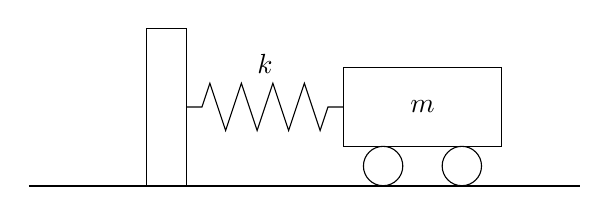
\begin{tikzpicture}
      \draw[fill=white] (-0.5,0) -- (-0.5,2) -- (0,2) -- (0,0);
      \draw[thick] (-2,0) -- (5,0);
      \draw[fill=white] (2,0.5) rectangle node {$m$} (4,1.5);
      \draw[fill=white] (2.5,0.25) circle (0.25);
      \draw[fill=white] (3.5,0.25) circle (0.25);
      \draw (0,1) -- (0.2,1) -- ++(0.1,0.3)
      -- ++(0.2,-0.6) -- ++(0.2,0.6)
      -- ++(0.2,-0.6) -- ++(0.2,0.6)
      -- ++(0.2,-0.6) -- ++(0.2,0.6)
      -- ++(0.2,-0.6) -- ++(0.1,0.3)
      -- (2,1);
      \draw (1,1.3) node[above] {$k$};
    \end{tikzpicture}
  \end{center}
\end{example}

\begin{solution}
  Let $x$ be the horizontal displacement of the car, measured in the
  left-to-right direction, and calibrated so that $x=0$ corresponds to
  the position of the car when the spring is in its relaxed state.
  By Hooke's law, $F=-kx$, and by Newton's second law,
  $F=mx''$. Putting these two equations together, we have
  \begin{equation*}
    mx'' = -kx,
  \end{equation*}
  or equivalently,
  \begin{equation*}
    x'' = -\frac{k}{m} x.
  \end{equation*}
  This is the equation of motion. By
  Theorem~\ref{thm:differential-equation}, the general solution is
  \begin{equation*}
    x = a\sin(\sqrt{\frac{k}{m}}\,t) + b\cos(\sqrt{\frac{k}{m}}\,t).
  \end{equation*}
  Thus, the car will periodically move left and right, with a
  frequency that is proportional to $\sqrt{k/m}$.  Note that in this
  problem, we have ignored other effects such as friction, which would
  eventually dampen the motion.
\end{solution}

% ----------------------------------------------------------------------
\subsection{A system of linear differential equations}

We now consider a system with more than one degree of
freedom. Consider a train made up of three cars of mass $m_1=1\kg$,
$m_2=2\kg$, and $m_3=1\kg$, which are aligned on a track and connected by
springs. Let us assume that each spring has the same spring constant
$k=1\frac{\SI{N}}{\m}$.
\begin{equation*}
    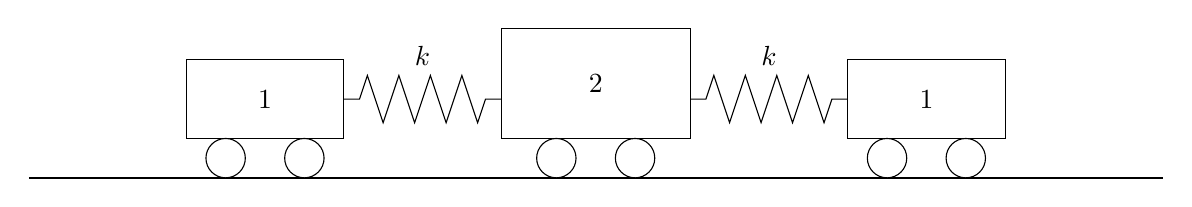
\begin{tikzpicture}
      \draw[thick] (0,0) -- (14.4,0);
      \begin{scope}
        \draw[fill=white] (2,0.5) rectangle node {$1\kg$} (4,1.5);
        \draw[fill=white] (2.5,0.25) circle (0.25);
        \draw[fill=white] (3.5,0.25) circle (0.25);
      \end{scope}
      \begin{scope}[xshift=4.2cm]
        \draw[fill=white] (1.8,0.5) rectangle node {$2\kg$} (4.2,1.9);
        \draw[fill=white] (2.5,0.25) circle (0.25);
        \draw[fill=white] (3.5,0.25) circle (0.25);
      \end{scope}
      \begin{scope}[xshift=8.4cm]
        \draw[fill=white] (2,0.5) rectangle node {$1\kg$} (4,1.5);
        \draw[fill=white] (2.5,0.25) circle (0.25);
        \draw[fill=white] (3.5,0.25) circle (0.25);
      \end{scope}
      \begin{scope}[xshift=4cm]
        \draw (0,1) -- (0.2,1) -- ++(0.1,0.3)
        -- ++(0.2,-0.6) -- ++(0.2,0.6)
        -- ++(0.2,-0.6) -- ++(0.2,0.6)
        -- ++(0.2,-0.6) -- ++(0.2,0.6)
        -- ++(0.2,-0.6) -- ++(0.1,0.3)
        -- (2,1);
        \draw (1,1.3) node[above] {$k$};
      \end{scope}
      \begin{scope}[xshift=8.4cm]
        \draw (0,1) -- (0.2,1) -- ++(0.1,0.3)
        -- ++(0.2,-0.6) -- ++(0.2,0.6)
        -- ++(0.2,-0.6) -- ++(0.2,0.6)
        -- ++(0.2,-0.6) -- ++(0.2,0.6)
        -- ++(0.2,-0.6) -- ++(0.1,0.3)
        -- (2,1);
        \draw (1,1.3) node[above] {$k$};
      \end{scope}
    \end{tikzpicture}
\end{equation*}
Let $x$ be the position of the first car, $y$ the position of the
second car, and $z$ the position of the third car. Moreover, let us
calibrate these variables so that each car's position is measured from
its resting point, i.e., $x=0$, $y=0$, and $z=0$ means that all three
cars are in their natural resting position where both springs are
relaxed.

Then the extension of the left spring is $y-x$, and therefore the
force acting on the leftmost car is
\begin{equation*}
  F_1 = k(y-x).
\end{equation*}
Note that we have not negated the force, because the spring is to the
right of the car.  Also, the extension of the right spring is $z-y$,
and therefore the force acting on the rightmost car is
\begin{equation*}
  F_3 = -k(z-y).
\end{equation*}
Finally, there are two forces acting on the middle car. They are
$-F_1$ (from the left spring) and $-F_3$ (from the right
spring). Thus, the total force acting on the middle car is
\begin{equation*}
  F_2  = -F_1-F_3 = -k(y-x)+k(z-y) = k(x-2y+z).
\end{equation*}
From Newton's second law, the acceleration of each car is given by
$m_1x'' = F_1$, $m_2y'' = F_2$, and $m_3z''=F_3$. We therefore have
the following equations of motion:
\begin{eqnarray*}
  x'' &=& \frac{k}{m_1}(y-x), \\
  y'' &=& \frac{k}{m_2}(x-2y+z), \\
  z'' &=& \frac{k}{m_3}(z-y). \\
\end{eqnarray*}
Notice that this not a single differential equation, but a system of
differential equations. Each of $x''$, $y''$, and $z''$ can
potentially depend on each of $x$, $y$, and $z$. Let's ignore the
physical units and plug in $k=1$, $m_1=1$, $m_2=2$, and $m_3=1$. The
equations now are:
\begin{eqnarray*}
  x'' &=& y-x, \\
  y'' &=& \frac{1}{2}(x-2y+z), \\
  z'' &=& z-y. \\
\end{eqnarray*}
Since the right-hand side is a linear function of $x$, $y$, and $z$,
we can write it as a matrix multiplication:
\begin{equation*}
  \begin{mymatrix}{c} x'' \\ y'' \\ z'' \end{mymatrix}
  =
  \begin{mymatrix}{ccc}
    -1 & 1 & 0 \\
    \frac{1}{2} & -1 & \frac{1}{2} \\
    0 & 1 & -1 \\
  \end{mymatrix}
  \begin{mymatrix}{c} x \\ y \\ z \end{mymatrix}.
\end{equation*}
If we let
\begin{equation*}
  \vect{v} = \begin{mymatrix}{c} x \\ y \\ z \end{mymatrix}
  \quad\mbox{and}\quad
  A = \begin{mymatrix}{ccc}
    -1 & 1 & 0 \\
    \frac{1}{2} & -1 & \frac{1}{2} \\
    0 & 1 & -1 \\
  \end{mymatrix},
\end{equation*}
this equation can be written compactly as $\vect{v}'' = A\vect{v}$.

% ======================================================================
\subsection{CONTINUE HERE...}

  A
differential equation of the form $ay''+by'+cy = 0$ is called a
(homogeneous second order) \textbf{linear differential equation}%
\index{differential equation!linear}. Note
that the equation {\eqref{eqn:differential1}} is of this form, with
$a=1$, $b=0$, and $c=1$. In this section, we will use linear algebra,
and in particular diagonalization, to solve systems of homogeneous
linear differential equations.

This type of behavior along with complex eigenvalues is typical of the
deviations from an equilibrium point in the Lotka Volterra system of
differential equations which is a famous model for predator-prey
interactions. These differential equations are given by
\begin{eqnarray*}
  x^{\prime } &=&x(a-by) \\
  y^{\prime } &=&-y(c-dx)
\end{eqnarray*}
where $a,b,c,d$ are positive constants. For example, you might have
$X$ be the population of moose and $Y$ the population of wolves on an
island.

Note that these equations make logical sense. The top says that the
rate at which the moose population increases would be $aX$ if there
were no predators $Y$.  However, this is modified by multiplying
instead by $(a-bY) $ because if there are predators, these will
militate against the population of moose.  The more predators there
are, the more pronounced is this effect. As to the predator equation,
you can see that the equations predict that if there are many prey
around, then the rate of growth of the predators would seem to be
high. However, this is modified by the term $-cY$ because if there are
many predators, there would be competition for the available food
supply and this would tend to decrease $Y^{\prime }$.

The behavior near an equilibrium point, which is a point where the
right side of the differential equations equals zero, is of great
interest. In this case, the equilibrium point is
\begin{equation*}
  x=\frac{c}{d}, y=\frac{a}{b}.
\end{equation*}
Then one defines new variables according to the formula
\begin{equation*}
  x+\frac{c}{d}=x,\ y=y+\frac{a}{b}.
\end{equation*}
In terms of these new variables, the differential equations become
\begin{eqnarray*}
  x^{\prime } &=&\paren{x+\frac{c}{d}} \paren{a-b\paren{y+\frac{a}{b}
                  }} \\
  y^{\prime } &=&-\paren{y+\frac{a}{b}} \paren{c-d\paren{x+\frac{c}{d}
                  }}.
\end{eqnarray*}
Multiplying out the right sides yields
\begin{eqnarray*}
  x^{\prime } &=&-bxy-b\frac{c}{d}y, \\
  y^{\prime } &=&dxy+\frac{a}{b}dx.
\end{eqnarray*}
The interest is for $x,y$ small and so these equations are essentially
equal to
\begin{equation*}
  x^{\prime }=-b\frac{c}{d}y,\ y^{\prime }=\frac{a}{b}dx.
\end{equation*}
Replace $x^{\prime }$ with the difference quotient
$\frac{x(t+h) -x(t) }{h}$ where $h$ is a small positive number and
$y^{\prime } $ with a similar difference quotient. For example one
could have $h$ correspond to one day or even one hour. Thus, for $h$
small enough, the following would seem to be a good approximation to
the differential equations.
\begin{eqnarray*}
  x(t+h) &=&x(t) -hb\frac{c}{d}y, \\
  y(t+h) &=&y(t) +h\frac{a}{b}dx.
\end{eqnarray*}
Let $1,2,3,\ldots$ denote the ends of discrete intervals of time
having length $h$ chosen above. Then the above equations take the form
\begin{equation*}
  \begin{mymatrix}{c}
    x(n+1) \\
    y(n+1)
  \end{mymatrix} =\begin{mymatrix}{cc}
    1 & -\frac{hbc}{d} \\
    \frac{had}{b} & 1
  \end{mymatrix} \begin{mymatrix}{c}
    x(n) \\
    y(n).
  \end{mymatrix}
\end{equation*}
Note that the eigenvalues of this matrix are always complex.

We are not interested in time intervals of length $h$ for $h$ very
small.  Instead, we are interested in much longer lengths of
time. Thus, replacing the time interval with $mh$,
\begin{equation*}
  \begin{mymatrix}{c}
    x(n+m) \\
    y(n+m)
  \end{mymatrix} =\begin{mymatrix}{cc}
    1 & -\frac{hbc}{d} \\
    \frac{had}{b} & 1
  \end{mymatrix} ^{m}\begin{mymatrix}{c}
    x(n) \\
    y(n)
  \end{mymatrix}.
\end{equation*}
For example, if $m=2$, you would have
\begin{equation*}
  \begin{mymatrix}{c}
    x(n+2) \\
    y(n+2)
  \end{mymatrix} =\begin{mymatrix}{cc}
    1-ach^{2} & -2b\frac{c}{d}h \\
    2\frac{a}{b}dh & 1-ach^{2}
  \end{mymatrix} \begin{mymatrix}{c}
    x(n) \\
    y(n)
  \end{mymatrix}.
\end{equation*}
Note that most of the time, the eigenvalues of the new matrix will be
complex.

You can also notice that the upper right corner will be negative by
considering higher powers of the matrix. Thus letting $1,2,3,\ldots$
denote the ends of discrete intervals of time, the desired discrete
dynamical system is of the form
\begin{equation*}
  \begin{mymatrix}{c}
    x(n+1) \\
    y(n+1)
  \end{mymatrix} =\begin{mymatrix}{rr}
    a & -b \\
    c & d
  \end{mymatrix} \begin{mymatrix}{c}
    x(n) \\
    y(n)
  \end{mymatrix},
\end{equation*}
where $a,b,c,d$ are positive constants and the matrix will likely have
complex eigenvalues because it is a power of a matrix which has
complex eigenvalues.

You can see from the above discussion that if the eigenvalues of the
matrix used to define the dynamical system are less than 1 in absolute
value, then the origin is stable in the sense that as
$n\rightarrow \infty$, the solution converges to the origin. If either
eigenvalue is larger than 1 in absolute value, then the solutions to
the dynamical system will usually be unbounded, unless the initial
condition is chosen very carefully. The next example exhibits the case
where one eigenvalue is larger than 1 and the other is smaller than 1.

The following example demonstrates a familiar concept as a dynamical system.
